\documentclass{article}
\usepackage{graphicx} 
\usepackage{tikz}% Required for inserting images
%\usepackage[letterpaper,top=2.54cm,bottom=2.54cm,left=3.17cm,right=3.17cm,marginparwidth=1.75cm]{geometry}
\usepackage[margin=1in]{geometry}
\usepackage{hyperref}
\usepackage{setspace}
\usepackage{amsmath}
\hypersetup{
    colorlinks=true,
    linkcolor=blue,
    filecolor=magenta,      
    urlcolor=cyan,
    pdftitle={Overleaf Example},
    pdfpagemode=FullScreen,
}

\title{Practical Concerns for Estimating Mixed Hidden Markov Models}
\author{}
\date{}

\doublespacing

\begin{document}

\maketitle

\section{Introduction}

The circadian rhythm plays a major role in regulating human health. 
Disruption of the wake/sleep cycle is associated with a variety of negative health outcomes. 
For instance, the International Agency for Research on Cancer states that the chance of developing 
certain types of cancers is greatly increased when the circadian rhythm is disturbed. 
Sleep studies are the current gold standard to evaluate sleep, however they are resource 
intensive and thus can only focus on small groups at a time. 
Therefore, it is difficult to get population level data on the circadian rhythm. 

The National Health Examination Survey (NHANES) is a collection 
of studies aiming to quantify the health of US civilians. 
Beginning in 1960, NHANES become a yearly study in 1999 where 
specific goals change year-to-year to focus on emerging issues. 
For two years in the mid 2010s, a representative sample for the 
US of 5,000 participants (for a total of 10,000) were 
given a wrist physical activity monitor (PAM) for 9 days. 
Among other metrics, these PAMs measured physical activity by the minute. 
This data offers a unique glimpse into the circadian rhythm for the US population as a whole.

The proliferation of personal PAMs offers an interesting insight into sleep health. 
Currently, a lengthy and expensive sleep study is needed in order to quantify the circadian rhythm. 
PAMs offer a possibility of gathering much larger amounts 
of data easily, however the data may not be as accurate. 
Although this is an exciting opportunity, there are two main challenges. 

Firstly, PAMs measures activity not sleep. Although there is a clear 
connection between the two, the specific relationship is not immediately apparent. 
High activity periods most likely indicate an underlying wake state, 
however periods of inactivity may be hard to classify. For example, 
activity data may look similar for sedentary wake activities 
and sleep (e.g. watching TV may appear similar sleeping). Additionally, 
during periods of very low activity, measurements may be below the limit of detection (LoD). 
We propose to use an extension of a hidden Markov model (HMM) to capture this behavior. 
The observed data will be the activity measurements from the PAM 
and the hidden Markov state will be the unobserved wake/sleep status.

The second complication is that activity levels are heterogeneous across 
the population. Previously this issue has been handled by either extending 
the Markov state space from wake and sleep to high activity wake, low activity
 wake, and sleep or by estimating the emission parameters independently for 
 each person. In the first scenario, active people would spend a larger 
 proportion of their wake time in the high activity wake state compared to 
 the low activity wake state.  This solution may cause more problems than it 
 solves as there is no agreed upon cut off for what constitutes low/high activity. 
 Additionally, this greatly increases the complexity of adding important covariates 
 to the Markov transition matrix. Estimating a 3x3 transition matrix is much 
 more difficult than a 2x2, causing feasibility issues when large amounts of 
 data are used. For the second approach, although estimating the emission parameters 
 independently allows a greater fit this too causes more issues than it solves. 
 As the number of participants increases so too does the number of parameters. 
 For datasets that do not have a large number of repeated measurements for each 
 person this approach will not work. Lastly, it is not clear how this can be 
 extrapolated to new data without re-estimation. Instead we propose a mixed 
 HMM (MHMM) \cite{Altman2007} with an individual level random effect for the 
 activity data in the wake state. This allows people to have different levels 
 of activity while keeping the interpretable and computation friendly two state structure.

This project focuses on practical concerns for estimation of a MHMM, with a 
focus on guidelines for estimating MHMMs. Specifically, we aim to answer whether 
a MHMM is necessary for state reconstruction, or if a HMM is sufficient. If a 
MHMM is necessary, we discuss how many support points are needed for the nonparametric 
density estimation for the emission distribution random effect (RE). Afterwards 
we apply a MHMM to the NHANES physical activity data.

\section{Methods}
\subsection{Notation}

Define the set $\{S_{i1}, ..., S_{iT}\}$ as the states of a first order Markov 
chain (MC) corresponding to the wake/sleep cycle. If person i at time t is awake 
we let $S_{it}=0$, otherwise if person i is asleep at time t then $S_{it}=1$. 
To account for detection limit issues, let $\delta_{it}$ be 0 when the activity 
measurement is below the LoD and person i is asleep, and 1 otherwise. Therefore, 
we assume that when we observe a measurement below the LoD, the person must be in 
the sleep state. As this is a first order MC, it can be completely described by 
an initial probability, $P_j=P(S_{i1} =j)$, and a transition matrix where entry 
ij is equal to $P_{ij}=P(S_{it}=j|S_{it-1}=i)$. Define the set $\{a_{i1}, ..., a_{iT}\}$ 
as the observed physical activity data from a PAM for patient i. For person i 
at time t, we refer to the probability of the activity measurement given the 
current wake/sleep state as the emission distribution. The activity measurement 
given the current wake/sleep status is independent of all other MC states, or 
equivalently $P(a_{it}|S_{i1}, ..., S_{iT}) = P(a_{it}|S_{it})$. Therefore the 
HMM can be completely described by the initial, transition, and emission probabilities.

To allow for covariates in the transition probabilities, we model the probability
of changing states with the inverse-logit or expit function. We have 
$q(it)_{01} = \text{expit}(X_{it}\beta_0)$ and $q(it)_{10} = \text{expit}(X_{it}\beta_1)$ 
where $X_{it}$ is a vector of covariates and $\beta_j$ is the corresponding covariate
parameters. This allows both fixed (e.g. race) and time varying (e.g. current time) 
covariates to influence the transition probabilities. In our simulation study we 
let $\beta_j = \{\beta_{j0}, ..., \beta_{j4}\}$ and $X_{it} = \{1, x_{it1}, ..., x_{it4}\}$, 
where $x_{it1}$ and $x_{it2}$ are fixed covariates equal to 1 if that covariate applies to 
person i. $x_{it3} = \text{cos}(\frac{2\pi t}{96})$ and $x_{it4} = \text{sin}(\frac{2\pi t}{96})$ 
are time varying to account for the cyclical nature of the circadian rhythm.  Any first 
order harmonic function with a period of 96 can be estimated. A period of 96 was chosen 
as this is equivalent to modeling each day in 15 minute chunks.

We assume that the activity data given the underlying wake/sleep state is normally 
distributed. When person i is asleep, we assume $a_{it}$ is drawn from a normal 
distribution centered at $\mu_1$ with variance $\sigma_1^2$. When person i is awake, 
we assume $a_{it}$ is drawn from a normal distribution centered at $\mu_0+u_i$ with 
variance $\sigma_0^2$. $u_i$ is an old-style random effect directly related to the 
mean wake activity of person i. We require that the distribution of $u_i$ (H) has 
mean 0, but place no other restrictions on it. This assumption can be relaxed, however 
it facilitates easy comparison between simulations later on. To be clear, we do not 
necessarily assume that H is a normal distribution. There is little precedent on how 
activity is distributed across the US population and we did not want to automatically 
assume that it was normally distributed. Later on we will conduct a simulation study 
where H is varied. By including a RE in the model, we use the term mixed HMM (MHMM) to describe this model. 


\subsection{Estimation}

Without applying any additional methods, the likelihood is written
as equation \ref{like1}. Inside of the square brackets, we evolve
through the Markov chain for person i, multiplying the initial, 
transition, and emission probabilities. As we do not know the 
underlying MC state, it is not clear yet how to calculate these 
probabilities as the wake/sleep states are not observed. As $u_i$ 
is a continuous individual level random effect, we must integrate 
over its support for each individual. This integral is complex 
and and may require numerical methods to solve, increasing the 
computation required. The next two subsections will detail how 
to calculate this likelihood. 

\begin{equation}\label{like1}
f(\textbf{a}|\theta) = \prod_{i=1}^n \int_U \sum_{{s_1}\cdots{s_T}} \biggr[ 
    P(S_{i1})=s_1\prod_{t=2}^T P(S_{it}=s_t|S_{it-1}=s_{t-1}) \times 
    \prod_{t=1}^T P(a_{it}|S_{it}=s_t,u_i)^{\delta_{it}} \biggr] dH(u_i)
\end{equation}

\subsubsection{Nonparametric Density Estimation (NPDE)}

To simplify the integral (as well as allowing future computations 
with the forward-backward algorithm), we will estimate the RE 
distribution, H, with a discrete random variable, $b_i$. A small 
number of support points are chosen where the mass put on support 
point l is $\pi_l$. This can equivalently be written as 
$P(b_i = r_l) = \pi_l$ where $r_l$ is support point l. Later on 
we will conduct a simulation study where the number of support 
points ranges from one to six. Conceptually, this can be thought 
of as estimating a discrete distribution using a histogram where 
each bar of the histogram is a support point and the mass put on 
each support point is the height of the bar. It is important to 
note that using one support point is equivalent to leaving out 
the RE and thus the MHMM reduces to a HMM. NPDE has been applied 
with success numerous times in various applications \cite{izenman1991}. 
Using this approach we can write the likelihood as follows: 

\begin{equation}\label{like2}
f(\textbf{a}|\theta) = \prod_{i=1}^n \sum_{l=1}^L \sum_{{s_1}\cdots{s_T}} \biggr[ 
    P(S_{i1})=s_1\prod_{t=2}^T P(S_{it}=s_t|S_{it-1}=s_{t-1}) \times 
    \prod_{t=1}^T P(a_{it}|S_{it}=s_t,b_i=r_l)^{\delta_{it}} \biggr] \pi_l
\end{equation}

the change from equation \ref{like1} to \ref{like2} is that 
the integral over the support of U becomes a sum over the number 
of support points, L. Thus the time needed to compute this 
likelihood scales linearly with L. Increasing L increases 
estimation accuracy, however it comes at a computational price. 
L must be chosen before estimation, and there are no clear 
guidelines on how to do so. 

\subsubsection{EM Algorithm}

The EM algorithm is an iterative technique to preform maximum likelihood 
estimation in the presence of latent variables \cite{Baum1970}. 
Each iteration of the algorithm alternates between an expectation (E) 
and maximization (M) step, where the likelihood is guaranteed to 
increase between each iteration. Once the likelihood increase 
between iterations become sufficiently small, we consider the 
algorithm converged and stop. For the E step, we calculate the 
expected value of the full data log likelihood conditional on the 
observed data. We then maximize this expectation in the M step. The 
complete data likelihood can be written down as if we knew the 
latent variables that are required for estimation. It can be written as: 

\begin{equation}\label{cdata}
\begin{split}
    f(\textbf{a},\textbf{S}, \textbf{b} | \theta)  = & \prod_{i=1}^n \prod_{j=0}^1 
        P(S_{i1}=j)^{I(S_{i1}=j)} \times \\
    & \prod_{i=1}^n \prod^T_{t=2} \prod_{k=0}^1 \prod_{j=0}^1  
        P(S_{it}=j|S_{it-1}=k)^{I(S_{it-1}=k,S_{t}=j)} \times \\ 
    & \prod_{i=1}^n\prod_{l=1}^L \prod^T_{t=1}\prod_{j=0}^1 
        P(a_{it}|S_{it}=j,b_i=r_l)^{I(S_{it}=j,b_i=r_l)\delta_{it}}\\
    & \prod_{i=1}^n\prod_{l=1}^L \pi_l^{I(b_i=r_l)}
\end{split}
\end{equation}

where I() is an indicator variable. We then take the expected 
value of the log of equation \ref{cdata}, conditioning on the 
observed data. The result is the expectation of the complete data 
log likelihood. Letting $p_j = P(S_{i1}=j)$, $p_{kj} = P(S_{it}=j|S_{it-1}=k)$, 
and $\pi_l = P(b_i=r_l)$ we can calculate the E step by calculating 
equation \ref{ecdata} using a modified version of the forward-backward
 algorithm, detailed in the next section.

\begin{equation}\label{ecdata}
\begin{split}
    \ell = E\big[\text{log f}(\textbf{a},\textbf{S}, \textbf{b} | \theta) | \textbf{a},\theta\big]  = 
        & \sum_{i=1}^n\sum_{j=0}^1P(S_{i1}=j|\textbf{a})\text{log }p_j + \\
    & \sum_{i=1}^n \sum^T_{t=2} \sum_{k=0}^1 \sum_{j=0}^1 
        P(S_{it-1}=k,S_{it}=j|\textbf{a})\text{log }p_{kj} + \\ 
    & \sum_{i=1}^n \sum_{l=1}^L \sum^T_{t=1}\sum_{j=0}^1 
        P(S_{it}=j,b_i=r_l|\textbf{a}) \delta_{it}\text{log}P(a_{t}|S_{it}=j, b_i=r_l) + \\
    &  \sum_{i=1}^n \sum_{l=1}^L P(b_i=r_l|\textbf{a}) \text{log }\pi_l 
\end{split}
\end{equation}

\subsubsection{Adapted forward-backward Algorithm}
To account for the random effect in the emission distribution 
we use a modified version of the forward-backward algorithm 
that conditions on the discrete RE for person i \cite{Maruotti2011}. 
The forward and backward quantities are calculated recursively as shown 
in equations \ref{fwd} and \ref{bkwd}. Thus we have the following quantities: 
$\alpha_{it}(j,r_l) = P(a_{i1}, ..., a_{it}, S_{it} = j | b_i=r_l)$ and 
$\beta_{it}(j,r_l) =  P(a_{it+1}, ..., a_{iT} | S_{it} = j,b_i=r_l)$. 
We can then calculate the required quantities for equations \ref{mu1} 
and \ref{pi} as shown by equations \ref{probl} and \ref{probs0}.
 
\begin{equation} \label{fwd}
\alpha_{it}(j,r_l) = \begin{cases}
    p_{j} f(a_{i1}|S_{i1}=j,r_l) & \text{if } t = 1 \\
    \sum_{k=0}^1 \alpha_{it-1} (k,b_l)p_{kj}P(a_{it}|S_{it}=j,b_i=r_l)^{\delta_{it}} 
        & \text{if } t > 1\\
\end{cases}
\end{equation}

\begin{equation} \label{bkwd}
\beta_{it}(j,r_l) = \begin{cases} 
    \sum_{k=0}^1p_{jk}P(a_{it+1}|S_{it+1}=k,b_i=r_l)^{\delta_{it}}\beta_{it+1}(k,r_l) 
        & \text{if } t < n \\
    1 & \text{if } t = n \\
\end{cases}
\end{equation}


\begin{equation}\label{proba}
\begin{split}
    P(\textbf{a}) & = \prod_{i=1}^n \sum_{l=1}^L 
        P(\textbf{a}|b_{i}=r_l)P(b_{i}=r_l) = 
    \prod_{i=1}^n \sum_{l=1}^L \sum_{j=0}^1 \alpha_{iT}(j,r_l)\pi_l 
\end{split}
\end{equation}

\begin{equation}\label{probl}
\begin{split}
    P(b_{i}=r_l|\textbf{a}) & = \frac{P(\textbf{a}|b_{i}=r_l)P(b_{i}=r_l)}{P(\textbf{a})} = 
    \frac{\sum_{j=0}^1 \alpha_{iT}(j,r_l)\pi_l }{P(\textbf{a})}  
\end{split}
\end{equation}

\begin{equation}\label{probs0}
\begin{split}
    P(S_{it}=0,b_{i}=r_l|\textbf{a}) = \frac{P(S_{it}=0,\textbf{a}|b_{i}=r_l)
        P(b_{i}=r_l)}{P(\textbf{a})} = 
    \frac{\alpha_{it}(0,r_l)\beta_{it}(0,r_l)\pi_l }{P(\textbf{a})} 
\end{split}
\end{equation}

\begin{equation}\label{probs1}
\begin{split}
    P(S_{it}=1|\textbf{a}) = 
    \frac{\sum^L_{l=1}P(S_{it}=1,\textbf{a}|b_{i}=r_l)
        P(b_{i}=r_l)}{P(\textbf{a})} = 
    \frac{\sum^L_{l=1}\alpha_{it}(1,r_l)\beta_{it}(1,r_l)\pi_l }{P(\textbf{a})} 
\end{split}
\end{equation}


\begin{equation}\label{probstran}
\begin{split}
    P(S_{it-1}=k,S_{it}=j|\textbf{a}) & = 
        \frac{P(S_{it-1}=k,S_{it}=j,\textbf{a})}{P(\textbf{a})} \\
    & = \frac{\sum^L_{l=1}\alpha_{it}(k,r_l) p_{kj} P(a_{it}|S_{it}=j, b_i=r_l)
        \beta_{it}(j,r_l)\pi_l }{P(\textbf{a})} 
\end{split}
\end{equation}



\subsubsection{Parameter Estimates}

 To maximize each parameter, we take the derivative with respect 
 to that parameter and set the derivative to 0. It is important 
 to note the modular nature of this method as the initial, 
 transition, emission, and mixing ($\pi_l$) probabilities can 
 be maximized independently. Using the previously described 
 adapted forward-backward algorithm, we can calculate equations 
 \ref{init}-\ref{pi}, which give closed form solutions for the 
 initial, emission, and mixing parameters. As we cannot observe 
 $\mu_0$ or $r_l$ individually, we cannot estimate either independently. 
 This does not pose an issue as the sum of the two quantities is 
 the necessary component for the model and can be estimated. We 
 will refer to $\nu_l$ as the cluster mean in future sections. 

\begin{equation}\label{init}
    \hat{p_j}  = \frac{\sum^n_{i=0} P(S_{i1}=0|\textbf{a})}{n}
\end{equation} 

\begin{equation}\label{mu0}
    \hat{\mu_0} + \hat{r_l} = \hat{\nu_l} = 
    \frac{\sum_{i=1}^n \sum_{t=1}^T a_{it}P(S_{it}=0,b_{i}=r_l|\textbf{a})}
    {\sum_{i=1}^n \sum_{t=1}^T P(S_{it}=0,b_{i}=r_l|\textbf{a})}
\end{equation} 

\begin{equation}\label{sig0}
    \hat{\sigma}_0^2 = 
    \frac{\sum_{i=1}^n \sum_{l=1}^L \sum_{t=1}^T 
        (a_{it}-\nu_l)^2 P(S_{it}=0,b_{i}=r_l|\textbf{a})}
        {\sum_{i=1}^n \sum_{l=1}^L \sum_{t=1}^T P(S_{it}=0,b_{i}=r_l|\textbf{a})}
\end{equation} 

\begin{equation}\label{mu1}
    \hat{\mu_1} = 
    \frac{\sum_{i=1}^n \sum_{t=1}^T a_{it}\delta_{it}P(S_{it}=1|\textbf{a})}
        {\sum_{i=1}^n \sum_{t=1}^T \delta_{it}P(S_{it}=1|\textbf{a})}
\end{equation} 

\begin{equation}\label{sig1}
    \hat{\sigma}_1^2 = 
    \frac{\sum_{i=1}^n \sum_{l=1}^L \sum_{t=1}^T 
        (a_{it}-\mu_1)^2 P(S_{it}=1|\textbf{a})}
        {\sum_{i=1}^n \sum_{l=1}^L \sum_{t=1}^T P(S_{it}=1|\textbf{a})}
\end{equation} 

\begin{equation}\label{pi}
    \hat{\pi_l} = \sum_{i = 1}^n \frac{P(b_i = r_l)}{n}
\end{equation}


Unlike the previous parameters, no closed form solution for 
the transition probabilities exist. Instead, we preform a 
single Newton-Raphson step on the derivative of the likelihood 
at each iteration of the EM algorithm. Thus, 
$\beta_{j}^* = \beta_{j} - (\frac{\partial^2\ell}{\partial \beta_{j}^2})^{-1}
\frac{\partial\ell}{\partial \beta_{j}}$, where $\beta_{j}$ is 
our current estimate and $\beta_{j}^*$ is our updated estimate. 

\section{Simulation Study Results}

As noted in the introduction, the goal of this paper is to 
supply guidelines for MHMM estimation. Namely, do MHMMs provide 
a substantial advantage compared to HMMs, and if so how many 
support points are necessary for the NPDE of the RE distribution. 
We have designed a simulation study to answer these questions.

For the simulation study, we first simulate the sequence of MC 
states corresponding to the wake/sleep state of person i at time 
t according to pre-specified initial and transition probabilities. 
We vary both the number of people (1000 and 5000) and the length 
of time per person (one day and one week of follow up). Then for 
each person we draw an individual level RE from its distribution H. 
We considered different underlying RE distribution such that H is 
normal, gamma, normal/gamma mixture, t with 2 degrees of freedom, 
and t with 3 degrees of freedom (figure \ref{REdist}). We then 
simulate the observed activity data where $a_{it} \sim N(2+u_i,3)$ 
if person i is awake at time t and $a_{it} \sim N(0,2)$ if person i 
is asleep at time t. The parameters of the MHMM were estimated, where 
the number of support points was varied from 1 to 6. Finally we use 
the Viterbi algorithm to construct the most likely sequence of 
wake/sleep states given our estimated parameters. We can then compare 
the estimated sequence with the true wake/sleep sequence. All of this 
was repeated 100 times for each combination (number of people, length 
of observation, choice of H).

\begin{figure}
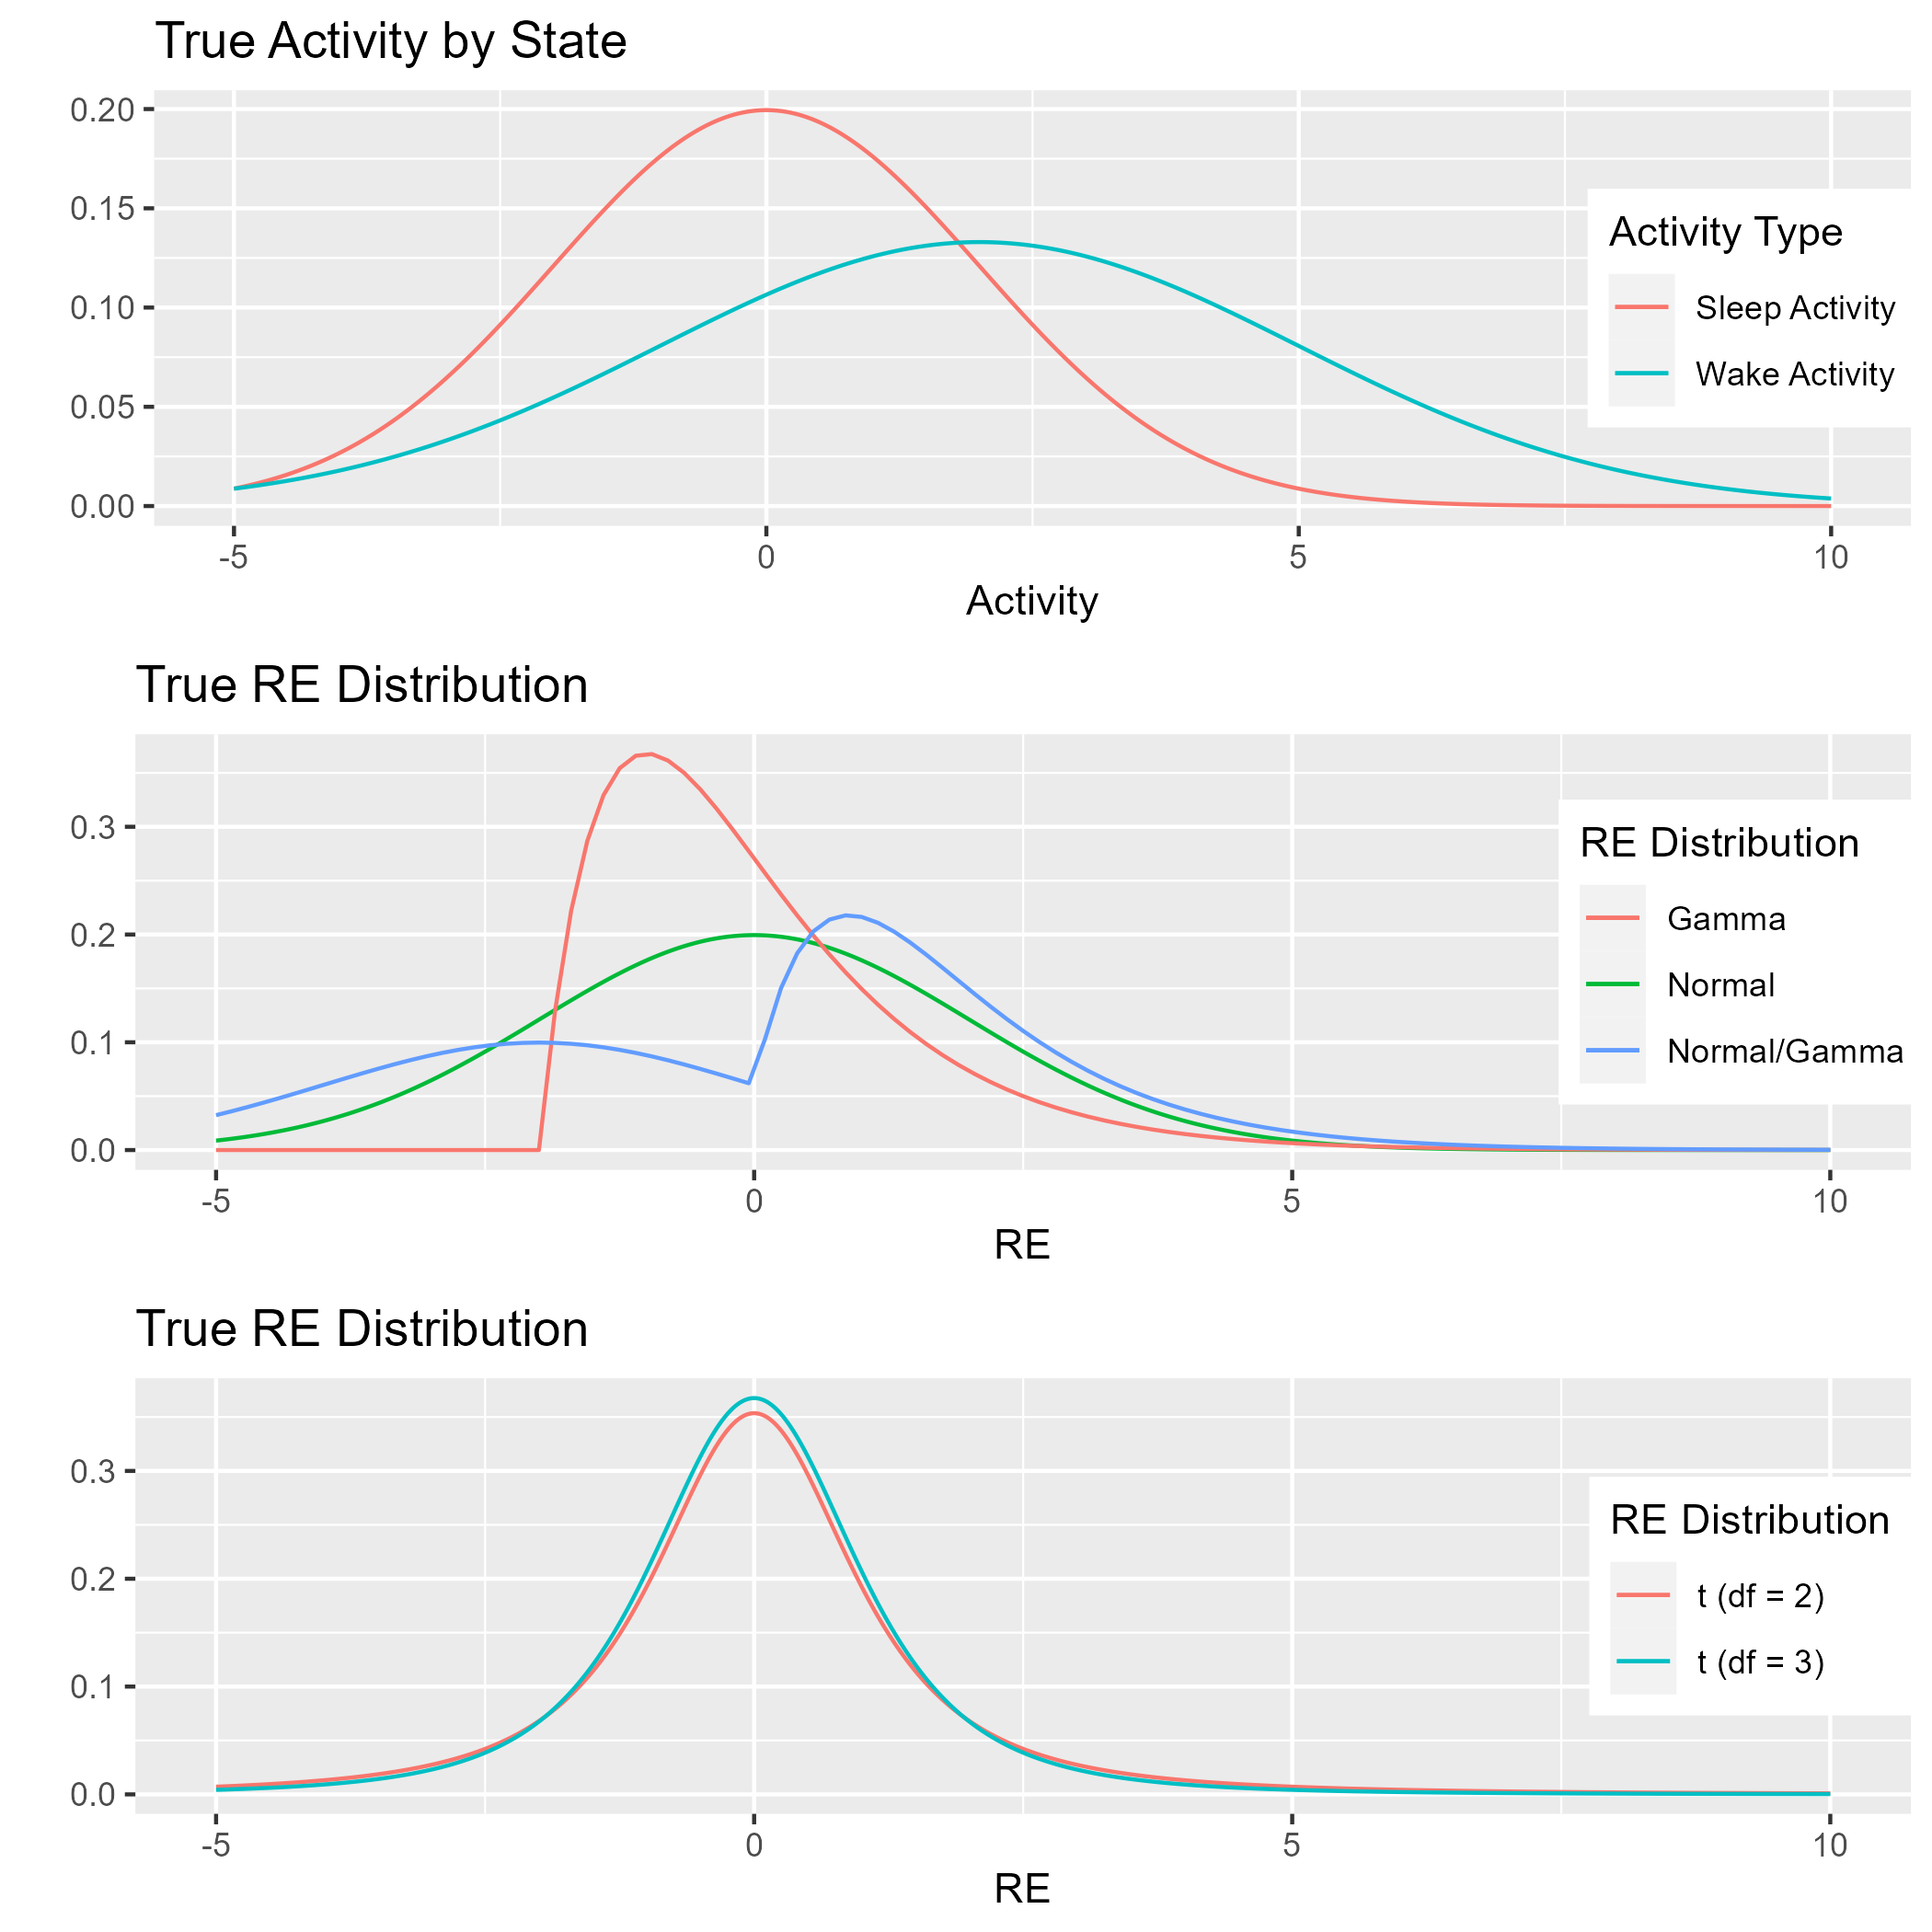
\includegraphics[scale=.5]{Support/REdist.png}
\centering
\caption{Distributions used in simulation study. Top plot shows wake 
(no RE) and sleep activity distribution. The bottom two plots show the 
different continuous RE distributions. RE distributions have been split 
up over two plots to increase readability.}
\label{REdist}
\end{figure}

The top plot of figure \ref{REdist} shows the wake (without a RE) and 
sleep activity distribution. Each individual's wake activity distribution 
would be shifted to the right or left depending on if $u_i$ is positive 
or negative. The bottom two plots show the different continuous RE 
distributions selected. The 5 choices for H have been split up into 
two plots to increase readability.

Figure \ref{NLacc} shows the results from the simulation. The y-axis 
for this figure is the percent agreement between the estimated wake/sleep 
sequence and the true wake sleep sequence. The color represents the 
number of support points, where the dark purple is one support point 
and the light green is 6. The x-axis represents the different simulation
settings (days of follow up, number of participants, and RE distribution). 
Taking the left most purple point, we can follow the line down and see 
that the point represents the percent of the wake/sleep sequence 
correctly predicted when the simulated data had 1 day of follow up, 1000 
participants, and the continuous RE comes from a gamma distribution.

As noted above, one support point is equivalent to leaving out the 
random effect, which in turn simplifies the mixed HMM to a standard HMM. 
As can be seen from figure \ref{NLacc}, as the purple line is the lowest, 
one support points has the lowest accuracy. This indicates that we see 
substantial accuracy gains from using a mixed HMM  (with any number 
of support points) compared to a standard HMM when there truly is a 
RE in the emissions distribution. We see that this accuracy increase 
is true for all simulation settings, meaning that the MHMM is more 
accurate than the HMM for all combinations of sample size and underlying RE distribution.

\begin{figure}
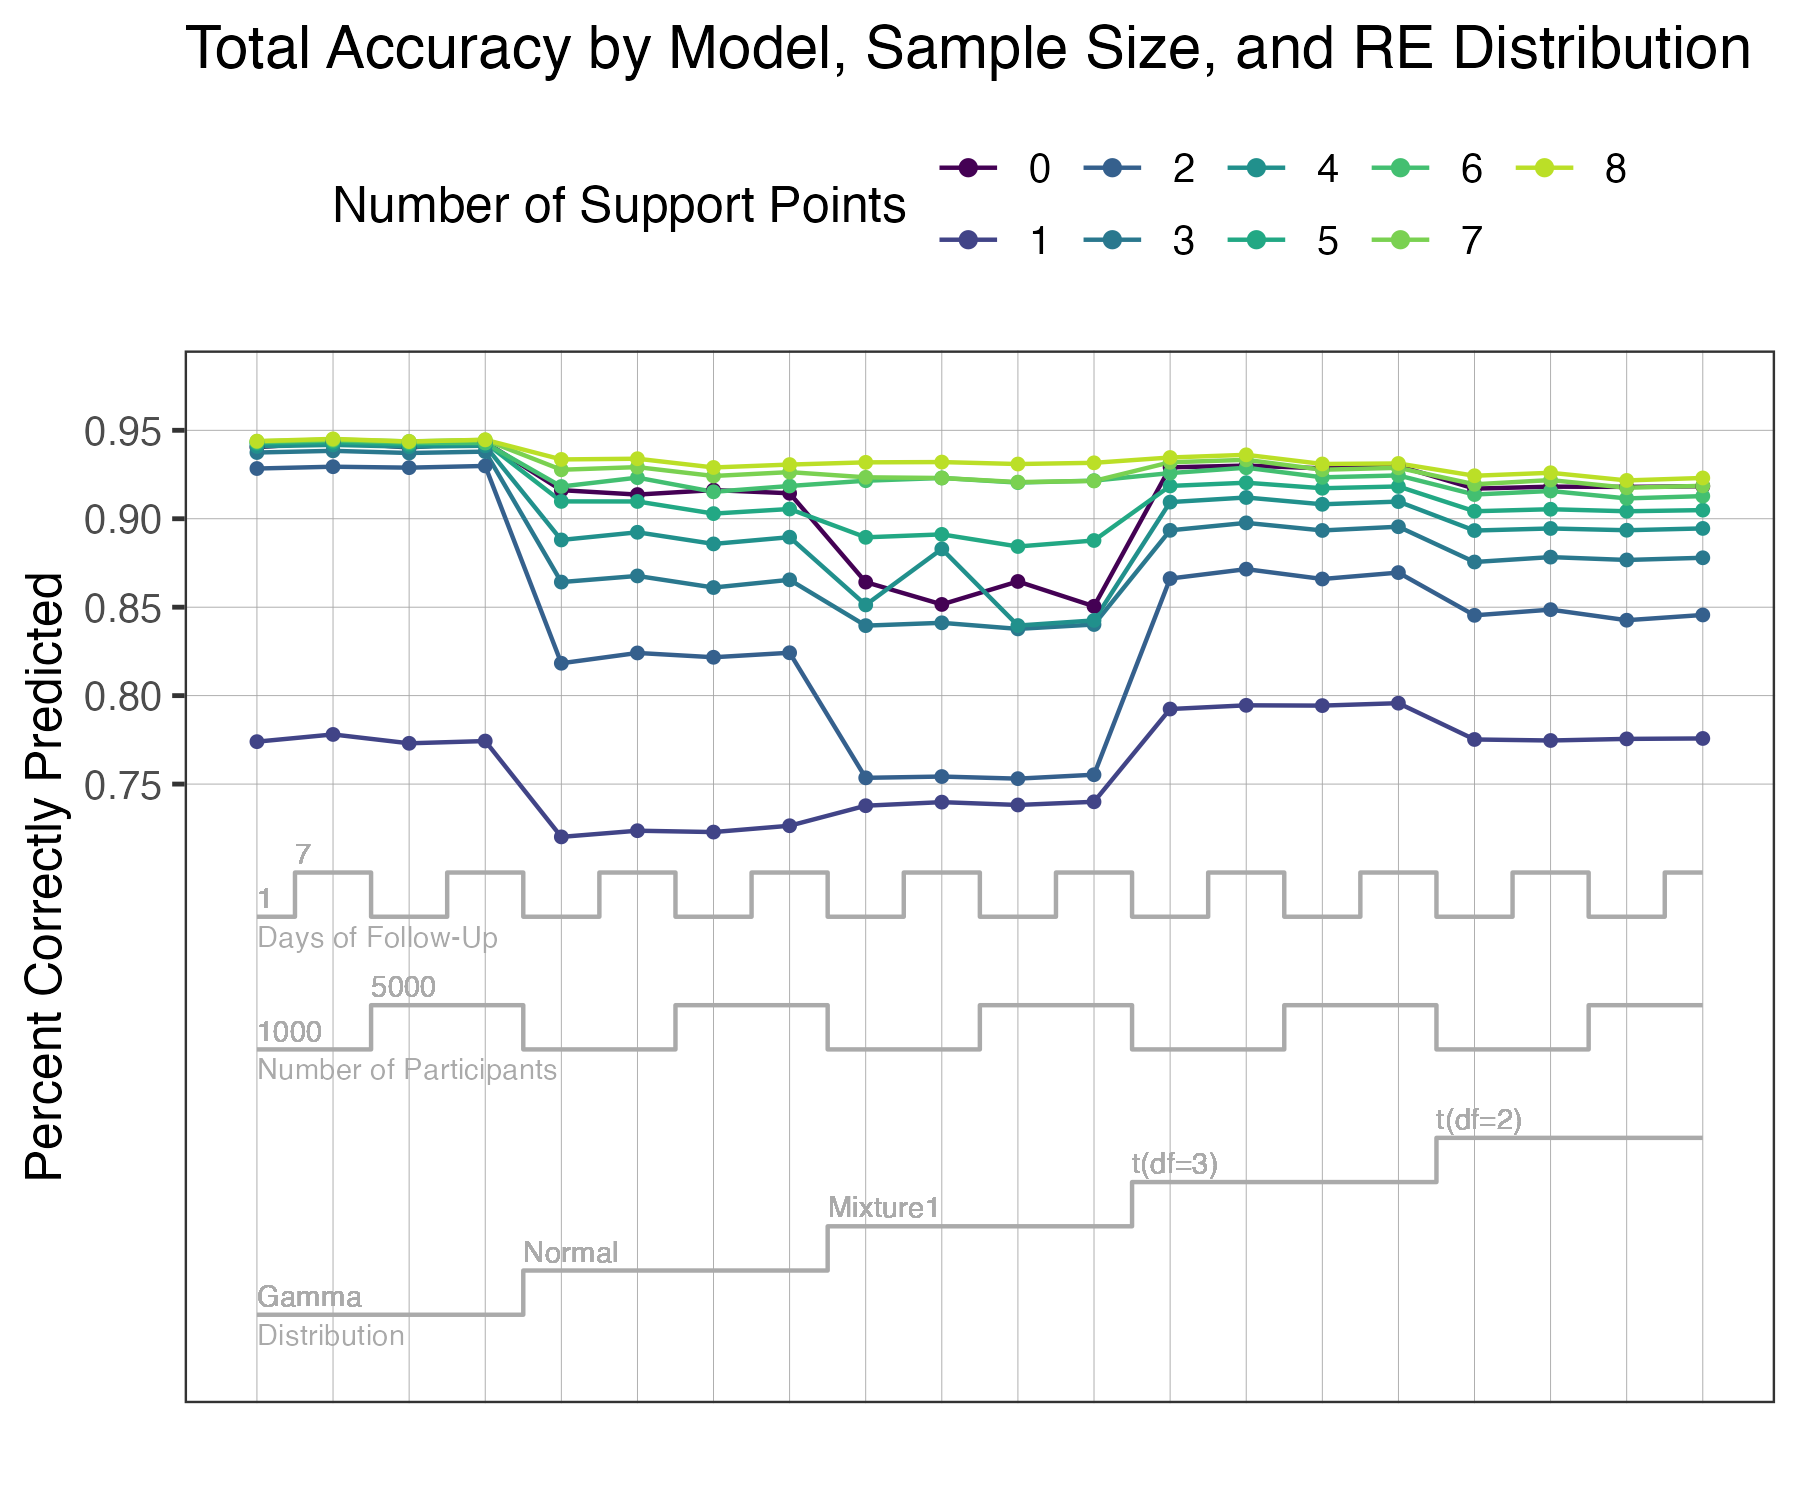
\includegraphics[scale=.8]{Support/NestedLoopAcc.png}
\centering
\caption{Nested loop plot of simulation results for total accuracy of predicted wake/sleep sequence. Each point is the median of 100 simulations and color indicates the number of support points. The X axis indicates the simulation settings, which are a combination of days follow-up, number of participants, and RE distribution.}
\label{NLacc}
\end{figure}

Our next question was about the number of support points needed 
for the NPDE of the RE. We see that this is mainly dependent upon 
the underlying continuous RE distribution and not the sample size 
in most situations. When H is gamma, two support points suffice. 
When H is normal, three support points may be preferred to two, 
but the returns diminish quickly after that. When H is a gamma/normal 
mixture, four support points are needed. For the t distributions, 
sample size plays a minor role as well. For a t distribution with 3 
degrees of freedom the trade off between computation time and number 
of support points needs to be evaluated as there are minimal, but present, 
differences for two, three, and four support points. For the 1 day of 
follow up with 5000 participants we see a large dip for two support points. 
This occurs because when the number of people increases, it is more 
likely that an extreme individual RE value is simulated. Thus one of
the support points is more likely to be placed to account for extreme 
values leaving only one support point to account for the remaining 
activity measurements. When increasing to a total of three support 
points, two can be used for the bulk and one for extreme values. 
A similar trend can be seen for a t distribution with two degrees 
of freedom, however, as the RE is even more spread out, more support 
points are necessary. A t distribution with two degrees of freedom 
may not be a realistic scenario, however figure \ref{NLacc} shows 
that with only 6 support points we can accurately predict the wake/sleep
 cycle under more extreme conditions. 

\begin{figure}
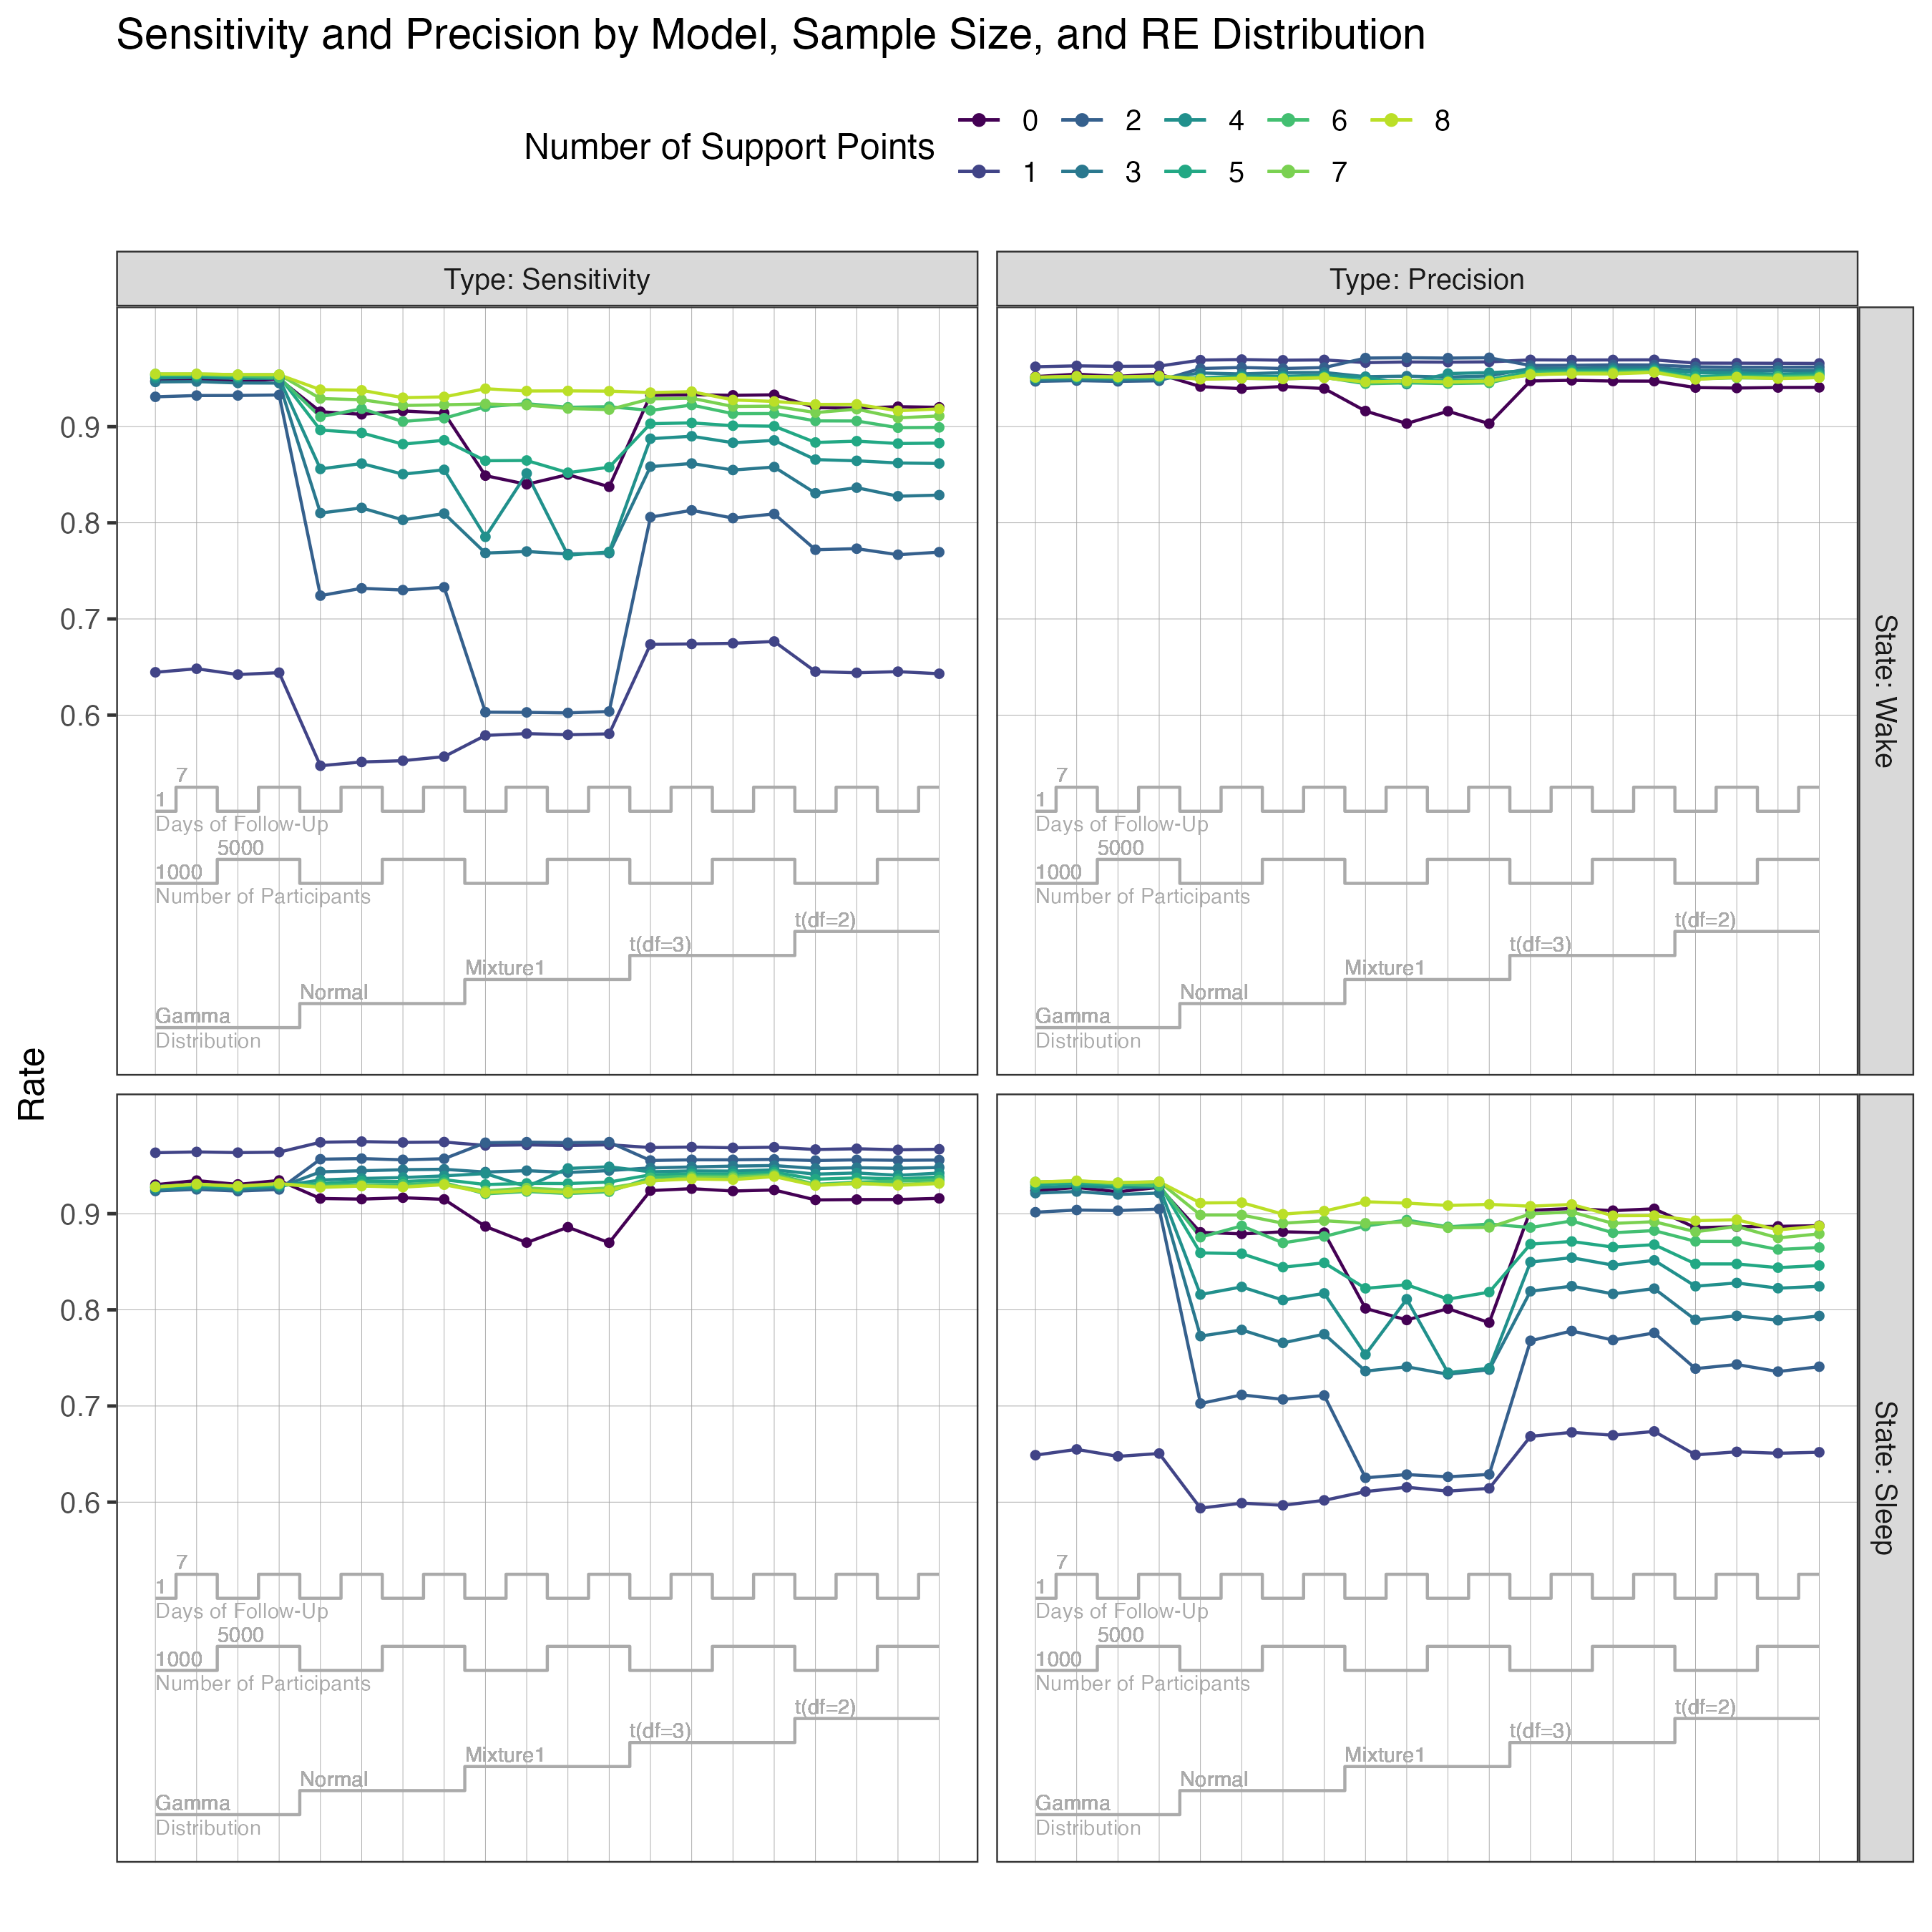
\includegraphics[scale=.65]{Support/NestedLoopSP.png}
\centering
\caption{Nested loop plot of simulation results for 
sensitivity (left column) and precision (right column) 
for wake (top row) and sleep (bottom row). Each point is
 the median of 100 simulations and the color indicates 
 the number of support points. The X axis indicates the 
 simulation settings, which are a combination of days follow-up, 
 number of participants, and RE distribution. Precision may also 
 be referred to as the positive predictive value.}
\label{NL2}
\end{figure}

To get a better understanding of how the method is working as a whole, 
we can look at metrics that are more specific than overall accuracy. 
Figure \ref{NL2} shows the sensitivity (left column) and precision 
(right column) for the wake (top row) and sleep (bottom row) states. 
Recall that wake sensitivity is the percent of all truly wake states 
that we accurately predict as wake, and wake precision is the percent 
of predicted wake states that are truly wake (this may also be referred 
to as the positive predictive value). When we fit a standard HMM 
(one support point) we see that although the sleep sensitivity is high, 
the wake sensitivity is very low. This is because unless the activity 
for time t is very high, the state at time t is predicted to be sleep. 
Therefore we are classifying all low activity wake behavior as sleep. 
This can be seen by looking at the precision. The sleep precision is 
very low because we classify truly wake states as sleep. On the other hand, 
wake precision is very high because although we rarely predict wake, 
when we do we are most likely correct as we only predict wake if we 
see a high activity measure.

When the number of support points is increased, the wake sensitivity 
increases, while the sleep sensitivity decreases. This occurs as 
although we are better at classifying sedentary wake activity as wake, 
we also  missclassify some sleep activity as wake. This causes wake 
precision to decrease and sleep precision to increase. Overall though, 
total accuracy is increased when the number of support points is increased 
as we can better classify wake states when we observe low activity measurements.


The number of support points needed depends on the spread of the 
underlying continuous RE distribution. When the spread is smaller, 
such as in the gamma simulation, two support points are sufficient. 
When the spread is larger, for instance as in the normal distribution, 
more support points are necessary. Looking closely at the 100 
simulations for 5000 people with a week of follow up when H is 
the normal distribution we can get a better sense of how increasing 
the number of support points increases overall accuracy. 
This simulation corresponds to the eighth column of points starting 
from the left in figure \ref{NLacc}. 

Figure \ref{CMM} contains information on the cluster mean 
$(\hat{\nu_l})$ in the top row and the mixing proportion 
$(\pi_l)$ in the bottom row. Each gray box indicated the 
total number of support points used in the model and the 
column of the plot is the specific support points starting 
with the first on the left and the last. Each boxplot 
incorporates data from 100 simulations. With one support point 
we have one cluster at around 3.75 and roughly 67\% accuracy. 
With two support points we still have a cluster at around 3.75 
and an additional cluster below 0. This new cluster around 0 is 
responsible for the ability to accurately predict the underlying 
state for sedentary people (i.e. those whose mean wake activity 
is similar to their sleep activity) and increases the overall 
accuracy to 75\%. However with these two support points, we may 
still inaccurately predict the underlying state when we observe 
a mean activity between 0 and 3.75. For instance, if we observe 
a mean activity of 2 for person i, it is unclear which cluster 
person i belongs to. When we use three support points the clusters 
are now at -.75, 2, and 4.5 and can accurately cover a wide range 
of mean wake activities. 

\begin{figure}
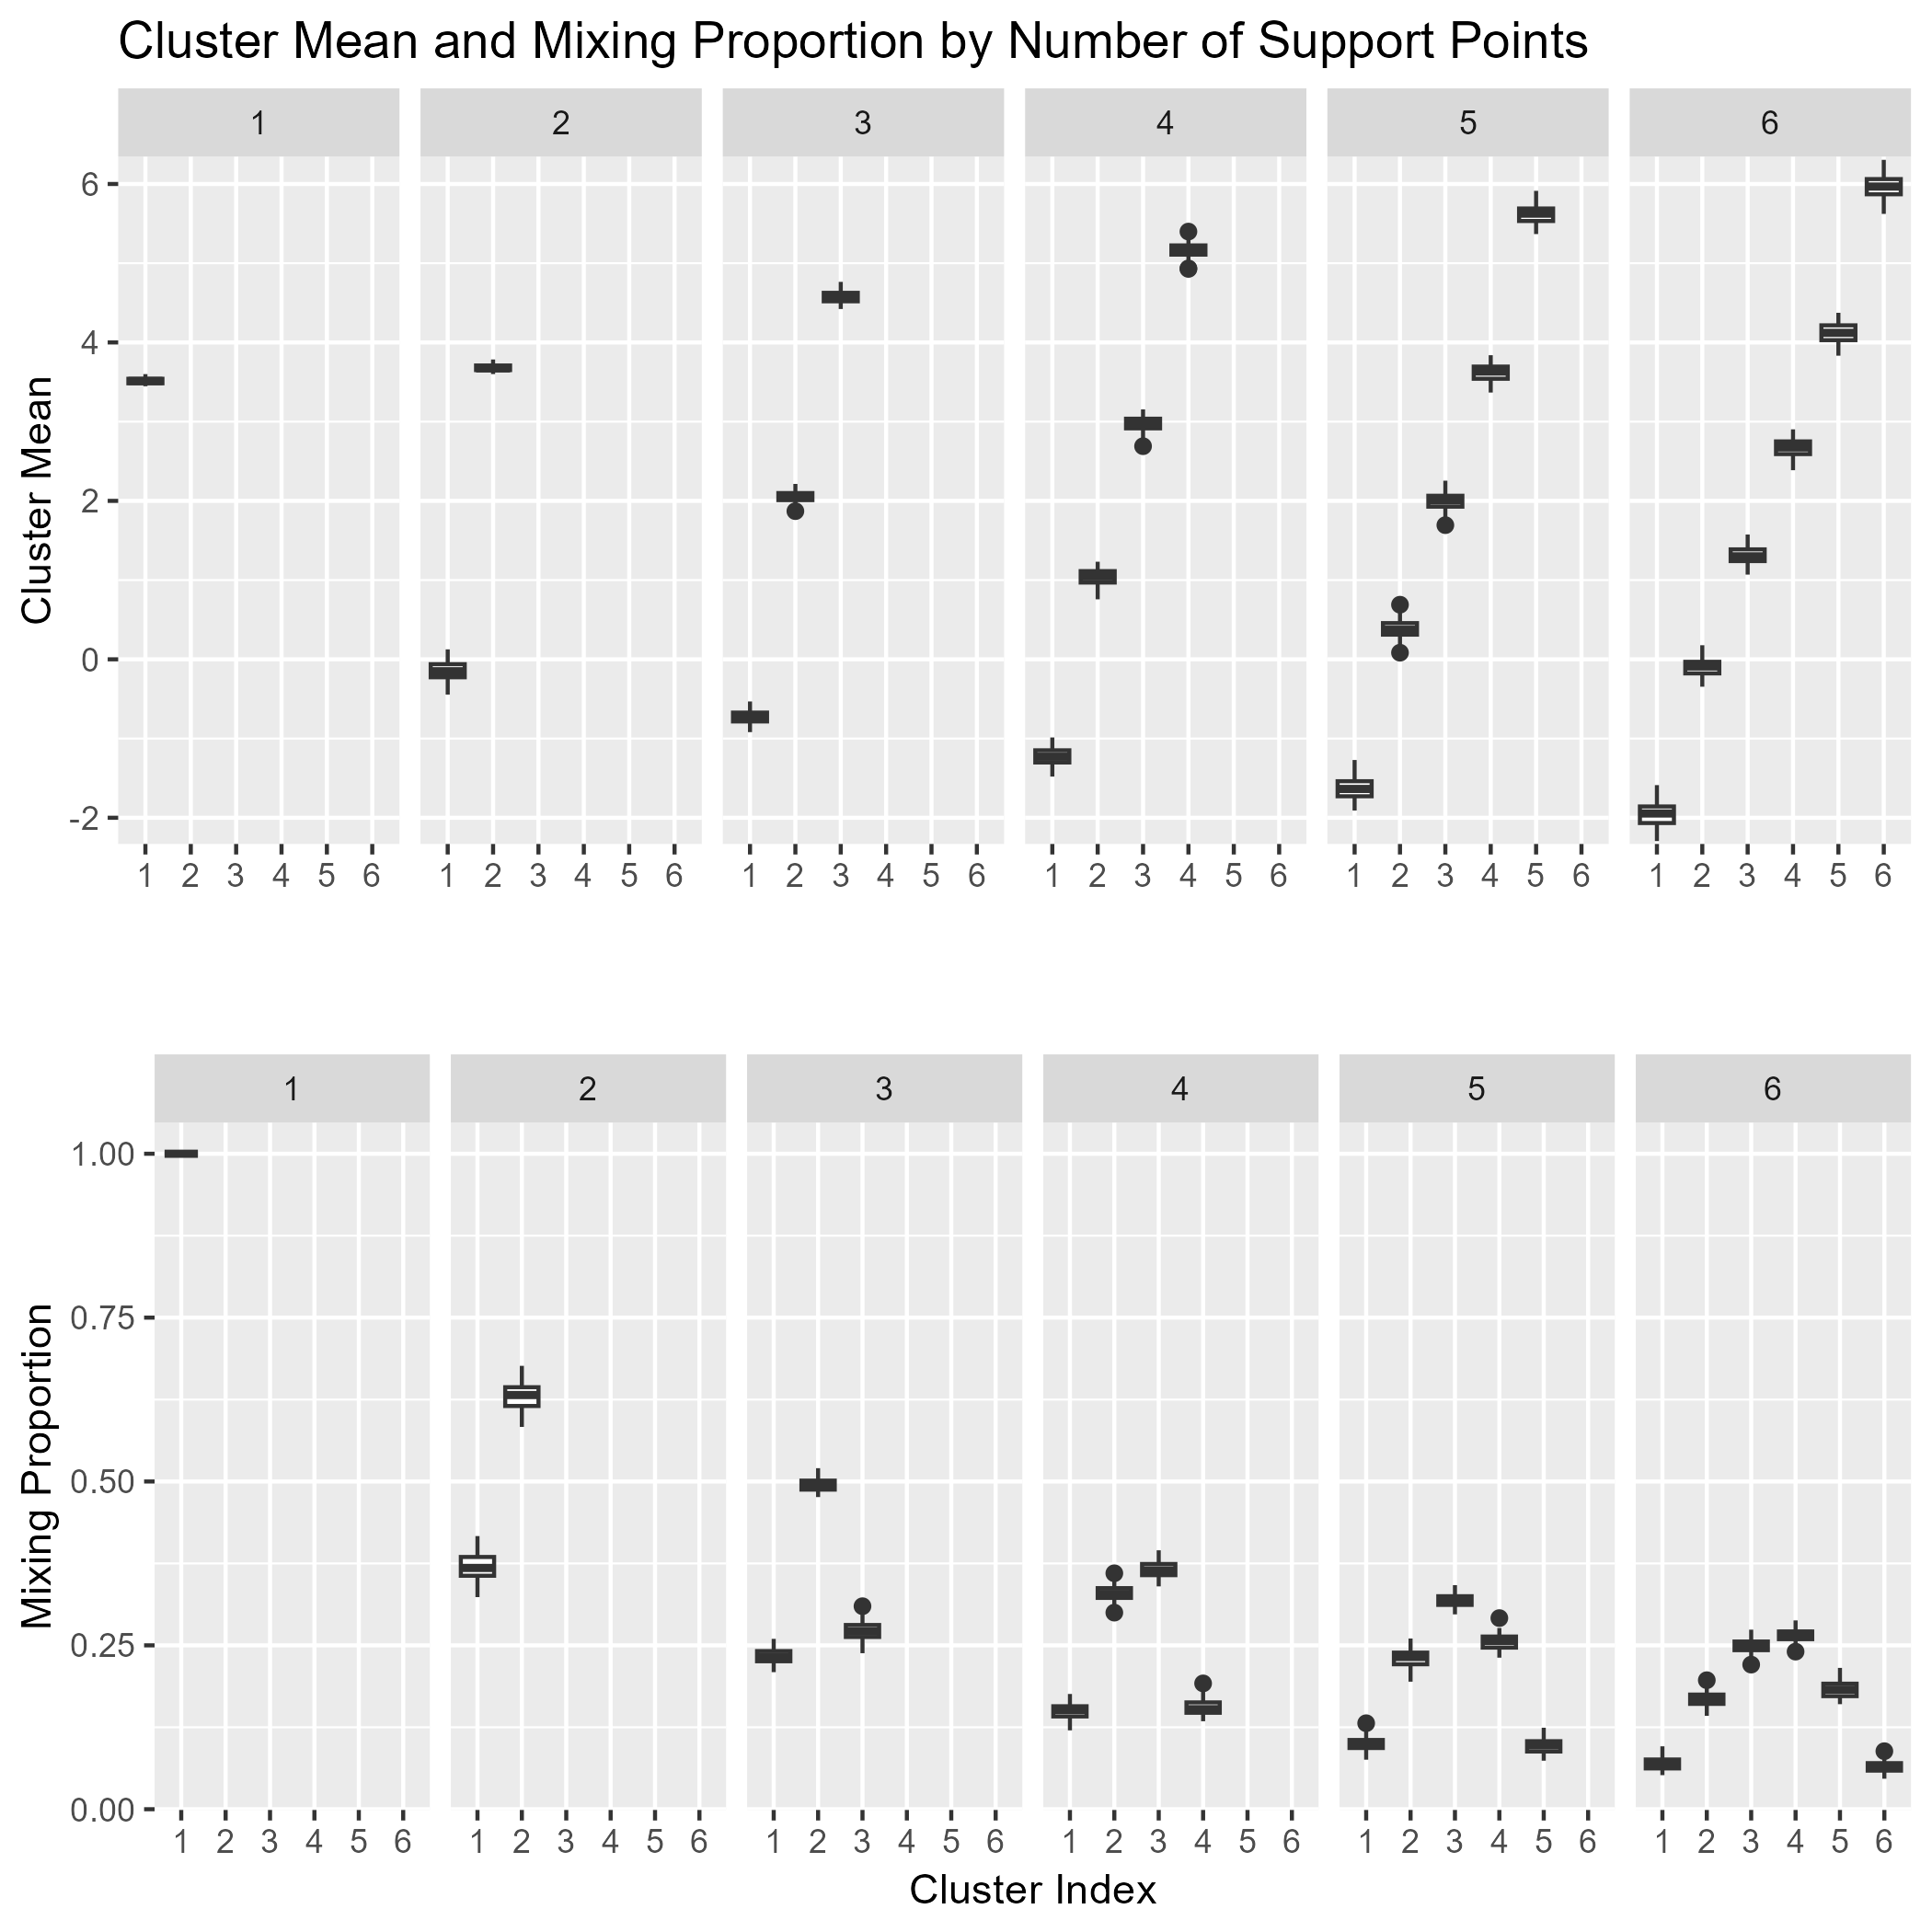
\includegraphics[scale=.48]{Support/clustmeanmix.png}
\centering
\caption{Cluster mean (top row) and mixing proportion (bottom row) 
for number of support points. Each column signifies the number 
of support points starting with one on the left and six on the right. 
Cluster mean represents $\nu_l=\mu_0+r_l$ and the mixing 
proportion is $r_l$. Each boxplot uses data from 100 simulations. }
\label{CMM}
\end{figure}

As noted before, there is a trade-off between the number of 
support points and computation time that must be balanced. 
Increasing the number of support points increases the accuracy 
of the state reconstruction, however there are diminishing returns. 
As the necessary computation time roughly scales linearly with 
the number of support points, it is pertinent that we choose enough 
support points to accurately estimate the sequence without 
significant computational burden. Figure \ref{time} is a nested 
loop plot showing the median running time in hours. We see that 
the increasing the number of support points generally increases 
the median running time. Additionally, for all of the simulations 
barring the t distribution with two degrees of freedom, two to 
four support points is sufficient for maximum accuracy as there 
is a steep drop off afterwards. For a t distribution with two 
degrees of freedom it may be beneficial to use six support points, despite the increased time.

\section{Conclusion}

Mixed hidden Markov models are a recent adaptation of HMMs 
which can account for individual level heterogeneity. In this 
paper we have shown that when the data is truly generated with 
a RE in the emissions distribution, a MHMM preforms much better 
than a HMM for state prediction. As the RE distribution is 
estimated using nonparametric density estimation, we have also 
shown that only a small number of support points are needed, 
where the exact number depends on the underlying continuous 
RE distribution. When this distribution has a higher variance, 
more support points are necessary for accurate state estimation. 
Although increasing the number of support points increases 
overall accuracy, it also increases the time needed to fit the model. 
Therefore, a balance must be found between accuracy and 
computation time. We suggest using two to four support points, 
as this provides both high accuracy and shorter running times. 


\begin{figure}
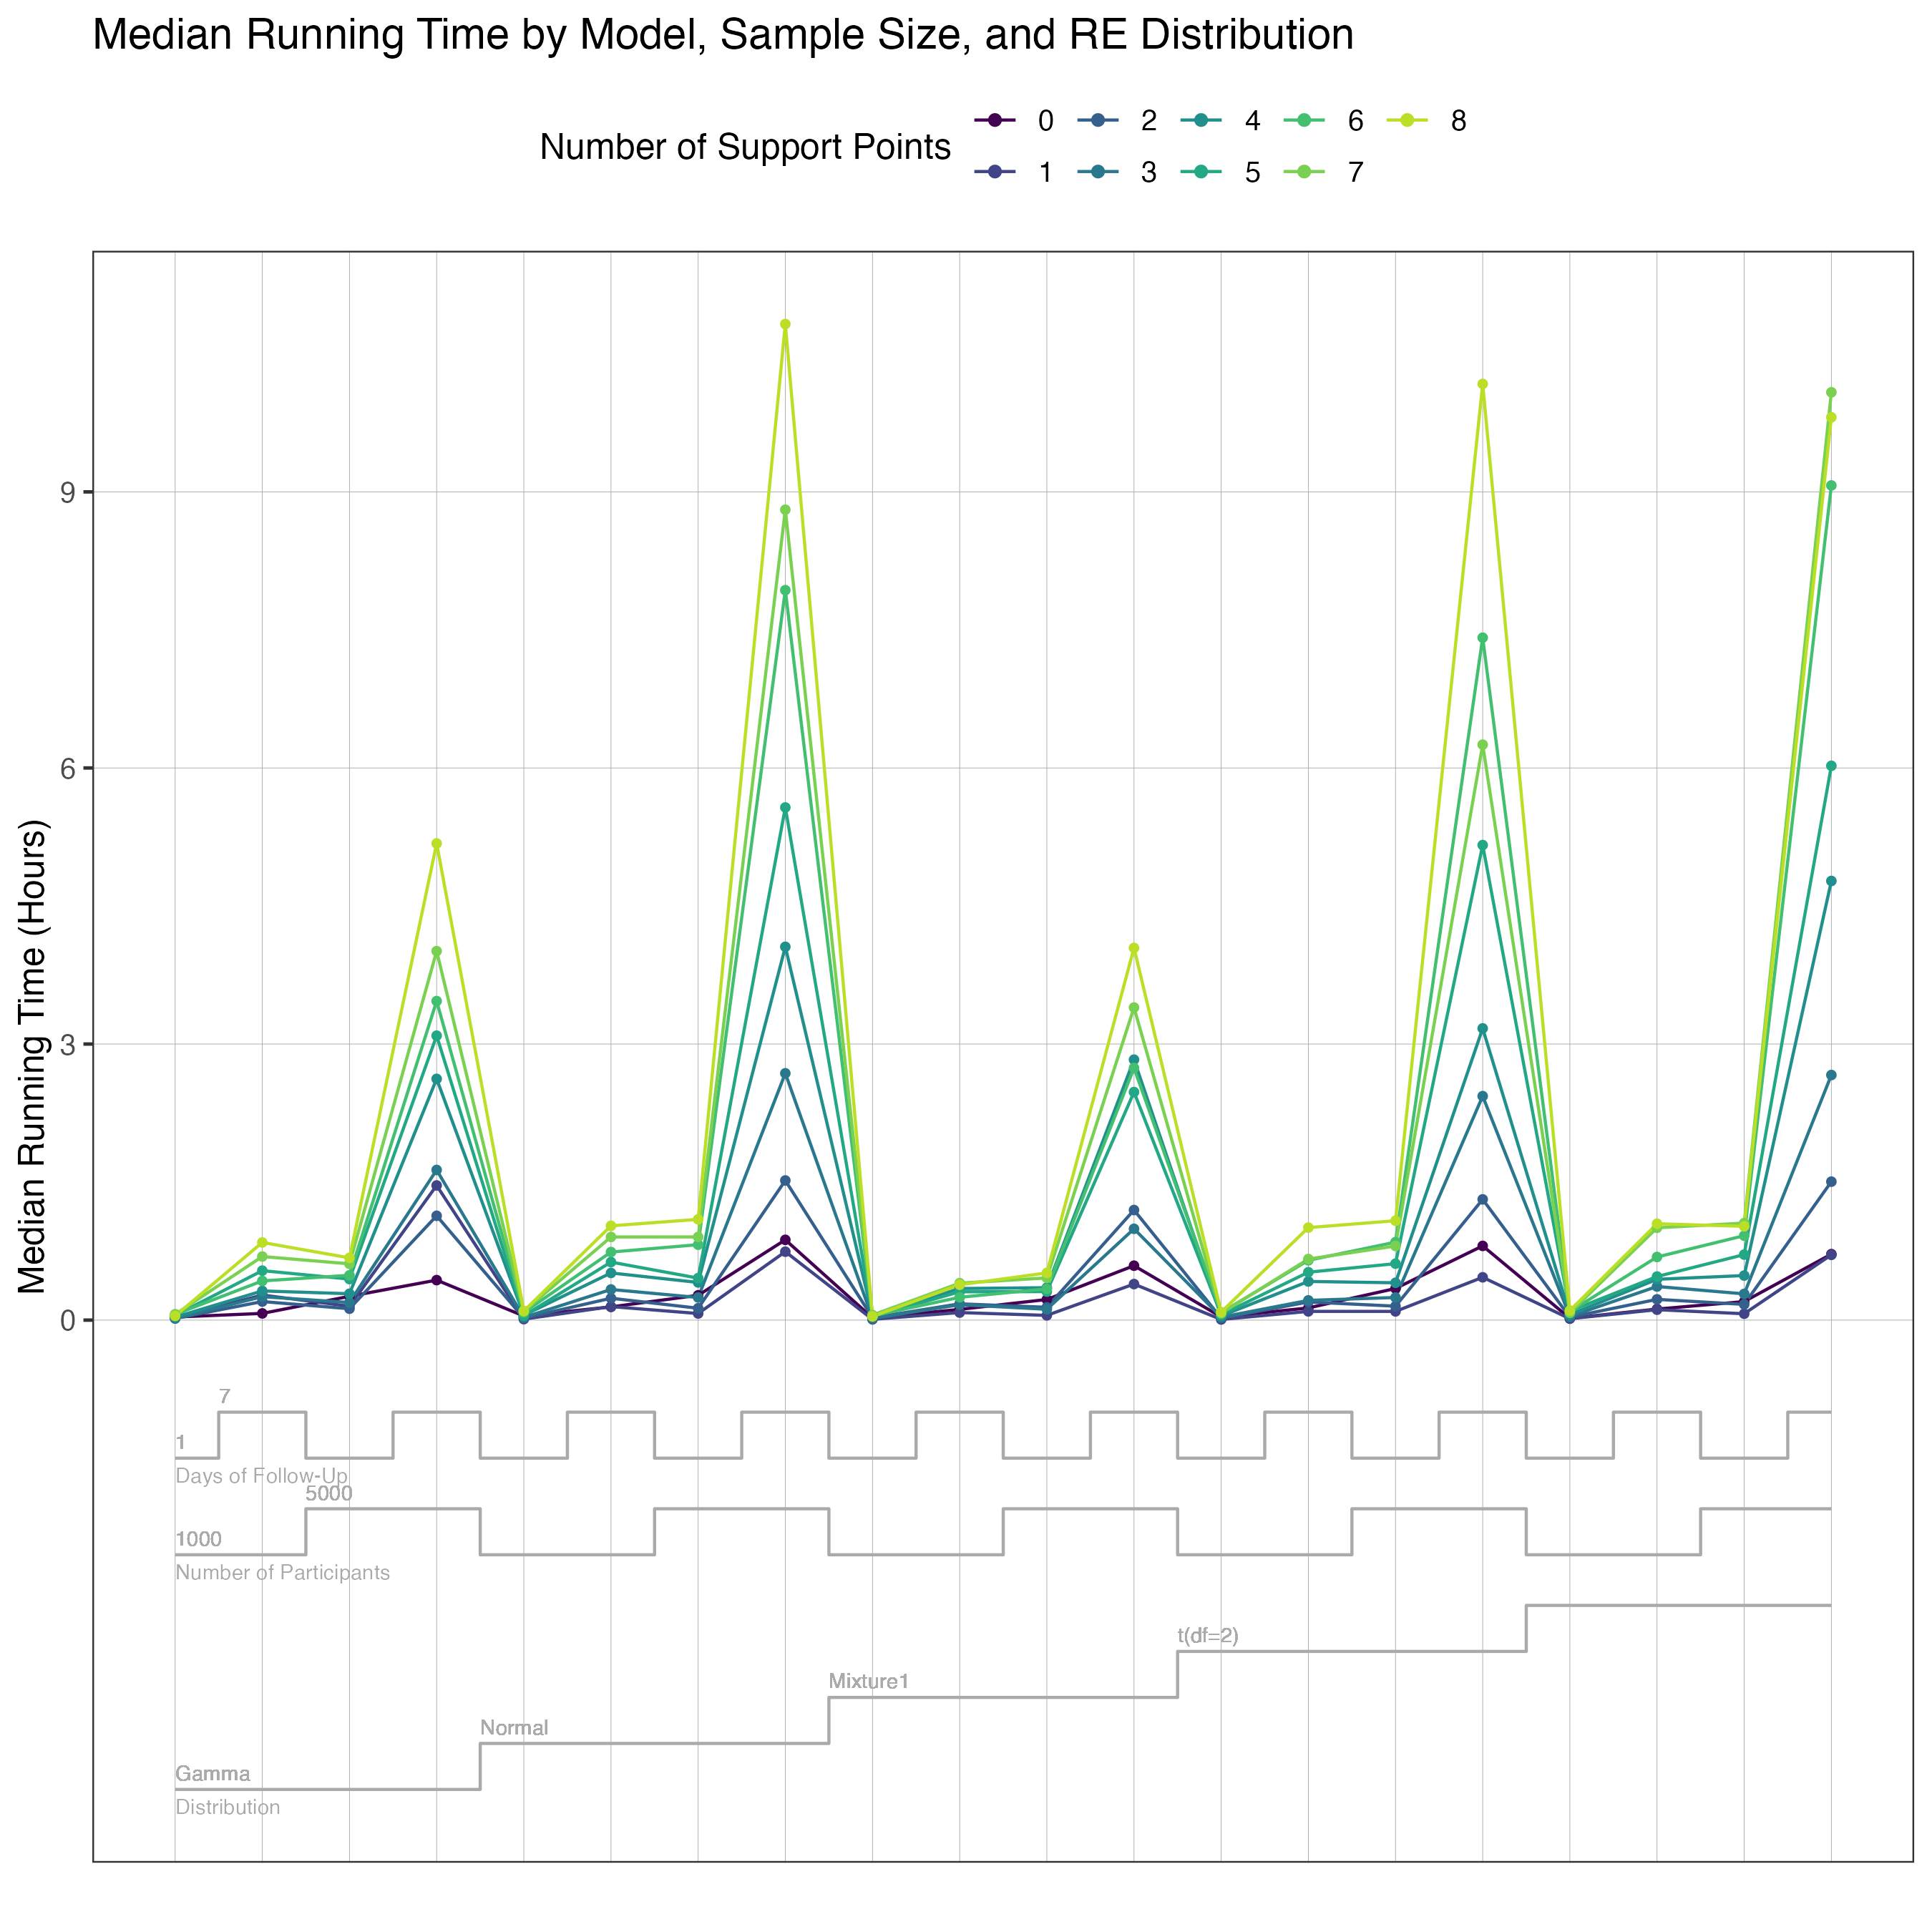
\includegraphics[scale=.55]{Support/NestedLoopCompTime.png}
\centering
\caption{Nested loop plot of simulation results for median 
running time in hours. Each point is the median of 100 simulations 
and the color indicates the number of support points. 
The X axis indicates the simulation settings, which is a 
combination of days follow-up, number of participants, and RE distribution.}
\label{time}
\end{figure}


\bibliographystyle{unsrt}
\bibliography{Support/sample}

\end{document}
